\documentclass[letterpaper,12pt]{article}

\usepackage{tabularx} % extra features for tabular environment
\usepackage{amsmath}  % improve math presentation
\usepackage{amssymb}
\usepackage{multirow}
\usepackage{xcolor}
\usepackage{gensymb}
\usepackage{appendix}
\usepackage{bigints}
\usepackage{mathtools}
\usepackage{gensymb}
\usepackage{float}
\usepackage{listings}
\usepackage[export]{adjustbox}
\usepackage[super]{nth}
\usepackage{graphicx} % takes care of graphic including machinery
\usepackage[margin=1in,letterpaper]{geometry} % decreases margins
\usepackage{cite} % takes care of citations
\usepackage[final]{hyperref} % adds hyper links inside the generated pdf file
\newcommand*{\tran}{^{\mkern-1.5mu\mathsf{T}}}
\DeclarePairedDelimiter\ceil{\lceil}{\rceil}
\DeclarePairedDelimiter\floor{\lfloor}{\rfloor}
\hypersetup{
    colorlinks=false,       % false: boxed links; true: colored links
    linkcolor=blue,        % color of internal links
    citecolor=blue,        % color of links to bibliography
    filecolor=magenta,     % color of file links
    urlcolor=blue         
}
%++++++++++++++++++++++++++++++++++++++++++++++++++++++++++++++++++++++++++++++++



%++++++++++++++++++++++++++++++++++++++++++++++++++++++++++++++++++++++++++++++++
% Start modifying the labwork number, your team number and the name and METU id
% of your group members.
\newcommand{\reporttitle}{Solution Set 5}
\newcommand{\reportauthor}{ Volkan Aydıngül (Id: 0075359 )\\
                            }
                            % If any teammate does not help to write this report,
                            % you may not write his/her name here.
%++++++++++++++++++++++++++++++++++++++++++++++++++++++++++++++++++++++++++++++++



%++++++++++++++++++++++++++++++++++++++++++++++++++++++++++++++++++++++++++++++++
% DO NOT MODIFY THIS SECTION
\begin{document}
\begin{titlepage}
\newcommand{\HRule}{\rule{\linewidth}{0.5mm}}
\begin{center} % Center remainder of the page
%	LOGO SECTION

\includegraphics[width = 8cm]{figures/koc_logo.png}

%	HEADING SECTIONS
\textsc{\Large PHYS 514 - Computational Physics}\\[1.5cm] 
%	TITLE SECTION
\HRule \\[0.6cm]
{ \huge \bfseries \reporttitle}\\ % Title of your document
\HRule \\[1.5cm]
\end{center}
\vspace{2cm}
%	AUTHOR SECTION
\begin{flushleft} \large
\textit{Author:}\\
\reportauthor% Your name
\end{flushleft}
\vspace{2cm}
\makeatletter
Date: \@date 
\vfill % Fill the rest of the page with whitespace
\makeatother
\end{titlepage}
%++++++++++++++++++++++++++++++++++++++++++++++++++++++++++++++++++++++++++++++++




\tableofcontents
\newpage





%\begin{figure}[H] 
%   \centering \includegraphics[width=\columnwidth]{figures/figure.png}           
%                \caption{Caption}                
%                   \label{fig:label}
%   \end{figure}

\section{Problem XIII}
\subsection{General Expression for Centered Finite Difference Stencils}
\paragraph{} Let's start to solve the problem by intuitive approach. To do this, we need to analyze a few \textit{Taylor expansions}. For example, let's investigate the following expansion:

\begin{equation}
    \label{eq:forward}
    f(x+h) = f(x) + hf^\prime(x) + \frac{h^2}{2!}f^{\prime\prime}(x) +  \frac{h^3}{3!}f^{\prime\prime\prime}(x)
\end{equation}

\begin{equation}
    \label{eq:backward}
    f(x-h) = f(x) - hf^\prime(x) + \frac{h^2}{2!}f^{\prime\prime}(x) -  \frac{h^3}{3!}f^{\prime\prime\prime}(x)
\end{equation}

\paragraph{}Substructing   \eqref{eq:backward} from   \eqref{eq:forward}, one can easily obtain that:
\begin{equation}
    \label{eq:firstderiv}
    f^\prime(x) = \frac{f(x+h) - f(x-h) }{2h} + \frac{h^2}{3!}f^{\prime\prime\prime}(x)
\end{equation}

\paragraph{} In   \eqref{eq:firstderiv}, the last term can be truncated, and can be written in the following final form:
\begin{equation}
    \label{eq:finafirstderiv}
    f^\prime(x) = \frac{f(x+h) - f(x-h) }{2h} + O(h^2)
\end{equation}

\paragraph{}  \eqref{eq:finafirstderiv} means that the error in the numerical calculation of the first derivative of function $f$ has an order of magnitude of $h^2$. Note that, this type of numerical derivative calculation is called central difference, because we expanded the function $f$ through two opposite direction from the center of $f$ (function itself). 

\paragraph{} Now, we need to observe a few things to proceed the derivation of a general rule. Firstly, we need to ask this question: What if we want to have $O(h)$ error? The answer is \textbf{we cannot}. Because, as can be seen from   \eqref{eq:firstderiv}, the $\frac{h^2}{2!}f^{\prime\prime}(x)$ terms are being canceled out. It is the \textit{natural} result that arises from the structure of the centered difference. We will elaborate on this in future discussion.

\paragraph{} Now, we can skip to the \textit{second} observation that we might have. To be able to obtain \nth{1} derivative with the error of $O(h^2)$, we expand the Taylor series about $3$ terms, including function itself and excluding the final to-be-truncated term. Therefore, we can \textit{naively} conclude that we need to have $n+m$ term to obtain $m^{th}$ derivative with the error of $O(h^n)$. Since one of the terms is for function itself, we can say that $n+m-1$ derivative term is sufficient to be extended. We can support this argument, actually, with a simple calculation. So far, we prepared a ground for the fact that if we want to have error of $O(h^n)$ for the calculation of $m^{th}$ derivative, we need to have $h^{m+n}$ term in the Taylor expansions. Let's illustrate this argument with an example. For example, we need calculate the \nth{3} derivative of a function, in this case, we will surely have several equation which includes $h^3$ term. In the same time, let's say we want to have error of $O(h^4)$. It is known that, at some point, we need to perform $\frac{h^7}{h^3}$ operation to have error of $O(h^4)$. Since, we are excluding the to-be-truncated term and including the function itself in the \textit{Taylor expansion}, it corresponds to $n+m$ needed term in the expansion, whose $n+m-1$ term is for derivative expressions. Note that we are excluding to-be-truncated term because our systematic approach required that. It means that another approach make use of this term and develop a method that includes it.

\paragraph{}Now, we can start to derive the general method for calculation of any derivative with the desired error. Before diving into the calculation, remember the above discussion we had about not being able to have \textit{odd} numbered error. The same type of irregularity can be also encountered when the derivative we will take is even numbered. Following above analogy, one can easily derive the reason also for that. All in all, we need to regulate our number of term expression according to it. Assume that $n$ is odd and we want error of $O(h^n)$, previously, we saw that even if we want this, we forcefully get $O(h^{n+1})$ error. Therefore, to write this in a more compact form, we can construct the following relation:

\begin{equation*}
    n\prime = 2 \floor{\frac{n+1}{2}}
\end{equation*}

If above relation is carefully investigated, one can conclude that $n\prime$ equals to the $n$ itself when $n$ is even number, and $n\prime$ equals to the $n+1$ itself when $n$ is odd number. Also, to deal with the irregularities in the degree of derivative, one can write the following relation:
\begin{equation*}
    2p+1 = 2\floor{\frac{m+n+1}{2}} - 1
\end{equation*}
where $2p+1$ is the number of terms that will be expanded during the Taylor series expansion. In this case, we also have $2p+1$ unknown. Doubtlessly, to solve $2p+1$ number of unknowns, we need to have $2p+1$ number of equations. We can construct that much linear equation by doing $p$ time forward expansion, $p$ times backward expansion, and, finally, by expressing function itself. However, most importantly, to be able to solve anything, we need to create a solvable form. We ca manage this by deducing following equation:

\begin{equation}
    \label{eq:generalform}
    f^{(m)}(x) =  \frac{a_{-p}f(x-ph) + a_{-(p-1)}f(x-(p-1)h) + \dots +  a_{p-1}f(x+(p-1)h) + a_{p}f(x+ph)}{h^m}
\end{equation}


where, for example, $f(x +  \Delta x)$ can be written in following form:
\begin{equation}
    \label{eq:taylorexp}
    f(x + \Delta x) = f(x) + ( \Delta x)f^\prime(x) + \frac{( \Delta x)^2}{2!}f^{\prime\prime}(x) +  \frac{( \Delta x)^3}{3!}f^{\prime\prime\prime}(x)+\dots+\frac{( \Delta x)^{2p}}{2p!}f^{(2p)}(x)
\end{equation}
\pagebreak
\paragraph{}When we combine  \eqref{eq:generalform} and \eqref{eq:taylorexp}, we can obtain:

\begin{equation}
    \label{eq:stencileqn}
    \begin{split}    
f^{(m)}(x)  = a_{-p}&\left[ f(x) + (-ph)f^\prime(x) + \frac{(-ph)^2}{2!}f^{\prime\prime}(x) + \dots+\frac{(-ph)^{2p}}{2p!}f^{(2p)}(x) \right] + \\
 a_{-(p-1)}&\left[ f(x) + (-(p-1)h)f^\prime(x) + \frac{(-(p-1)h)^2}{2!}f^{\prime\prime}(x) +\dots+\frac{(-(p-1)h)^{2p}}{2p!}f^{(2p)}(x) \right]\\
 &\vdots\\
 a_0&\left[f(x)\right]\\
 &\vdots\\
 a_{p-1}&\left[ f(x) + ((p-1)h)f^\prime(x) + \frac{((p-1)h)^2}{2!}f^{\prime\prime}(x) +\dots+\frac{((p-1)h)^{2p}}{2p!}f^{(2p)}(x) \right]\\
 a_{p}&\left[ f(x) + (ph)f^\prime(x) + \frac{(ph)^2}{2!}f^{\prime\prime}(x) + \dots+\frac{(ph)^{2p}}{2p!}f^{(2p)}(x) \right] / h^m
\end{split}
\end{equation}

\paragraph{}Looking at \eqref{eq:stencileqn}, one can deduce that all the coefficienct in front of the derivative terms and function itself should be zero, except the derivative term we are looking for. Therefore, we can write this relation in the matrix form as following:

\begin{equation*}
    \begin{bmatrix}
        1 & 1 & \dots & 1 & 1\\
        -(p) & -(p-1) & \dots & (p-1) & (p) \\
        (-p)^2 & (-(p-1))^2 & \dots & (p-1)^2 & (p)^2 \\  
        & & \vdots & & \\   
        & & \vdots & & \\   
        (-p)^{2p-1} & (-(p-1))^{2p-1} & \dots & (p-1)^{2p-1} & (p)^{2p-1} \\ 
        (-p)^{2p} & (-(p-1))^{2p} & \dots & (p-1)^{2p} & (p)^{2p} \\ 
    \end{bmatrix}
    \begin{bmatrix}
        a_{-p} \\
        a_{-(p-1)} \\
        a_{-(p-2)} \\
        \vdots \\
        a_{(p-2)} \\
        a_{(p-1)} \\
        a_{p} \\
    \end{bmatrix} = 
    \begin{bmatrix}
        0 \\
        0 \\
        \vdots \\
        m! \\
        \vdots \\
        0 \\
        0\\
    \end{bmatrix}
\end{equation*}

where $m!$ located on the $(m+1)^{th}$ on the RHS vector. Now, it is clear that the solution above linear system yields the required stencils for the $m^{th}$ derivative of function $f$ with the error of $O(h^n)$. Finally, we can calculat the derivative using \eqref{eq:generalform}.

\subsection{General Expression for Arbitrary Finite Difference Stencils}
\label{sec:arbitstencil}
\paragraph{}Similarly, we can write:


\begin{equation}
    \label{eq:generalformarb}
    f^{(m)}(x) = a_1f(x+s_1) + a_2f(x+s_2) + \dots +  a_{N-1}f(x+s_{N-1}) + a_{N}f(x+s_N)
\end{equation}

where $N$ is the number of stencils, and $m$ is order of derivative we want to take. Note that, to be able to construct such relation, the following inequality must be hold:
\begin{equation*}
    m<N
\end{equation*}

\paragraph{}Then, the following form can be constructed:

\begin{equation}
    \label{eq:stencileqnarb}
    \begin{split}    
f^{(m)}(x)  = a_{1}&\left[ f(x) + (s_1)f^\prime(x) + \frac{(s_1)^2}{2!}f^{\prime\prime}(x) + \dots+\frac{(s_1)^{N-1}}{(N-1))!}f^{(N-1)}(x) \right] + \\
 a_{2}&\left[ f(x) + (s_2)f^\prime(x) + \frac{(s_2)^2}{2!}f^{\prime\prime}(x) +\dots+\frac{(s_2)^{N-1}}{(N-1)!}f^{(N-1)}(x) \right]\\
 &\vdots\\
 a_{N-1}&\left[ f(x) + (s_{N-1})f^\prime(x) + \frac{(s_{N-1})^2}{2!}f^{\prime\prime}(x) +\dots+\frac{(s_{N-1})^{N-1}}{(N-1)!}f^{(N-1)}(x) \right]\\
 a_{N}&\left[ f(x) + (s_N)f^\prime(x) + \frac{(s_N)^2}{2!}f^{\prime\prime}(x) + \dots+\frac{(s_N)^{N-1}}{(N-1)!}f^{(N-1)}(x) \right] 
\end{split}
\end{equation}

Finally, from \eqref{eq:stencileqnarb}, we can construct the linear system in the matrix form:

\begin{equation*}
    \begin{bmatrix}
        s_1^0 & s_2^0 & \dots & s_{N-1}^0 & s_N^0\\
        s_1^1 & s_2^1 & \dots & s_{N-1}^1 & s_N^1\\
        s_1^2 & s_2^2 & \dots & s_{N-1}^2 & s_N^2\\
        & & \vdots & & \\   
        & & \vdots & & \\   
        s_1^{N-2} & s_2^{N-2} & \dots & s_{N-1}^{N-2} & s_N^{N-2}\\
        s_1^{N-1} & s_2^{N-1} & \dots & s_{N-1}^{N-1} & s_N^{N-1}\\
    \end{bmatrix}
    \begin{bmatrix}
        a_{1} \\
        a_{2} \\
        a_{3} \\
        a_{4} \\
        \vdots \\
        a_{N-1} \\
        a_{N} \\
    \end{bmatrix} =
    \begin{bmatrix}
        0 \\
        0 \\
        \vdots \\
        m! \\
        \vdots \\
        0 \\
        0\\
    \end{bmatrix}
\end{equation*}

where $m!$ located on the $(m+1)^{th}$ on the RHS vector. Now, it is clear that the solution above linear system yields the required stencils for the $m^{th}$ derivative of function $f$ with the error of $O(h^n)$. Finally, we can calculat the derivative using \eqref{eq:generalformarb}.

\section{Problem XIV}
\paragraph{} From now on, in all subsequent sections and subsections, there are analysis of the effect of the halving step size. In these calculations, a predetermined \textit{scale factor} used for each calculation scheme. Below, the calculation method for these scale factor can be found.
\paragraph{} Suppose that we have a truncation error of $O(h^n)$ for a given numerical calculation scheme, then the following relation can be written:
\begin{equation*}
    \label{eq:generictrun}
    \Phi_h = \Phi + Mh^n    
\end{equation*} 
\paragraph{} In \eqref{eq:generictrun}, the $\Phi_h$ represents a generic numerical operation. It could be differentiation or integration, it does not matter. Also, the $\Phi$ represents the real analytical result of this operation. Now, let's calculate this relation for a halved stepsize, then:

\begin{equation*}
    \Phi_{\frac{h}{2}} = \Phi + M\frac{h^n}{2^n}
\end{equation*}

And, again:

\begin{equation*}
    \Phi_{\frac{h}{4}} = \Phi + M\frac{h^n}{4^n} 
\end{equation*}

Then, one can naturally inspect the following relation:

\begin{equation*}
    \frac{\Phi_h - \Phi_{\frac{h}{2}}}{\Phi_{\frac{h}{2}} - \Phi_{\frac{h}{4}}} = \frac{Mh^n\left(1 - \frac{1}{2^n}\right)}{M\frac{h^n}{2^n}\left(1 - \frac{1}{2^n}\right)}
\end{equation*}
\paragraph{} In conclusion, it can be found out that:

\begin{equation*}
    \frac{\Phi_h - \Phi_{\frac{h}{2}}}{\Phi_{\frac{h}{2}} - \Phi_{\frac{h}{4}}} = 2^n
\end{equation*}

In all subsequent section, the scale factor is calculated using this relation.
\subsection{Numerical Differentiation}
\begin{figure}[H]
\centerline{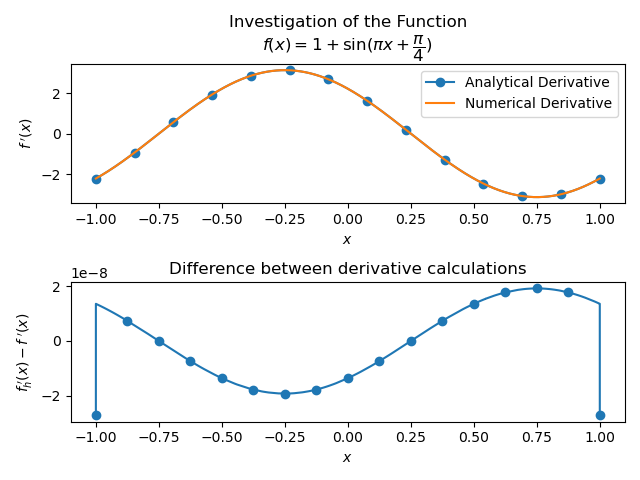
\includegraphics[width=\linewidth]{figures/14-1.png}}
\caption{Analytical and Numerical Derivative of the Function}
\label{fig:14-1}
\end{figure}

\paragraph{} In Figure \ref{fig:14-1}, the alignment of the numerical differentiation with analytical one can be observed. In numerical differentiation, the centered differentiation with 3 point stencil, which yields $O(h^2)$ accuracy, was chosen. As can be seen from Figure \ref{fig:14-1}, in this scheme, it is possible to have an error of $10^{-8}$, which can be seen as acceptable in this case.

\paragraph{} In Figure \ref{fig:14-2}, the effect of the step size on the error rate is investigated. It is known that, in numerical differentiation and integration operation, there are two types of error which accompanies all the time. These are truncation and round-off errors. However, both of these are not equally dominant all the time. When the step size is not so small, the majority of the error comes from the truncation error. However, when the  step size decreased enough, the round-off error comes into play. As can be seen from Figure \ref{fig:14-2}, until a certain value of step size, the error among the successive numerical differentiation calculations are similar. However, after a certain point, the dramatic decrease in the step size results in the striking increase in the relative error between successive differentiation calculations. Therefore, the blue jiggling noisy curve is obtained in Figure \ref{fig:14-2}.

\begin{figure}[H]
\centerline{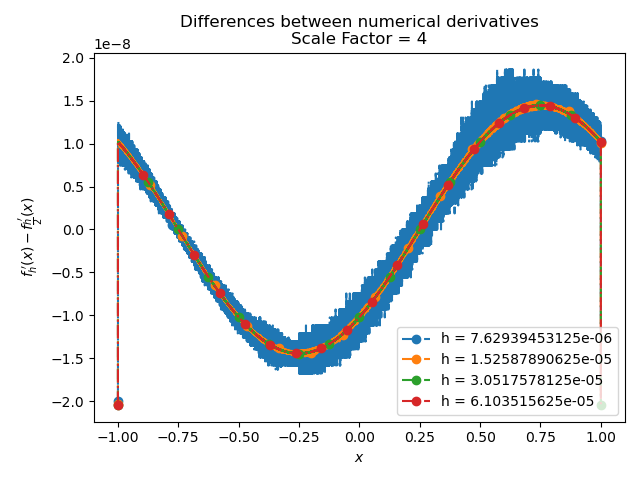
\includegraphics[width=\linewidth]{figures/14-2.png}}
\caption{Effect of Step Size on Error Rate}
\label{fig:14-2}
\end{figure}


\subsection{Numerical Integral}

\paragraph{} In Figure \ref{fig:14-3} the results of the analytical and the numerical integral can be observed. Also, it can be observed that while the \textit{Trapezoidal rule} yields relatively smooth error characteristics, it is not the case for the \textit{Simpson's method}. The resultant error due to the \textit{Simpson's method} displays a quite noisy behavior. Also, this noisy behavior can be observed in Figure \ref{fig:14-4-1}. The error between successively halved integral calculation shows a rambunctious behavior for the case of \textit{Simpson's method}, while, again, it is not the case for \textit{Trapezoidal rule}, see Figure \ref{fig:14-4-0} 
\begin{figure}[H]
\centerline{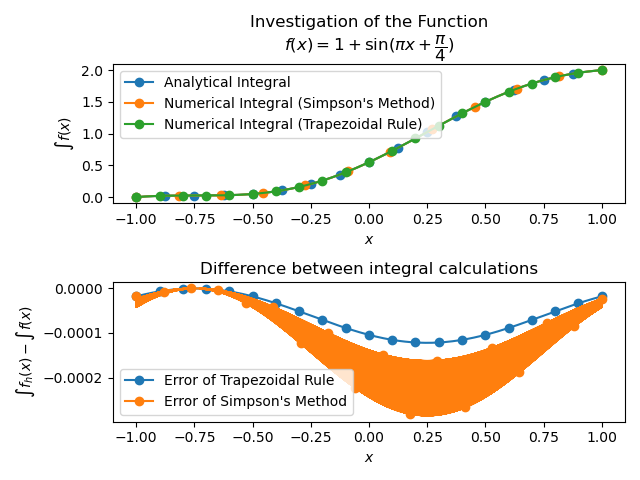
\includegraphics[width=1.0\linewidth]{figures/14-3.png}}
\caption{Analytical and Numerical Integral of the Function}
\label{fig:14-3}
\end{figure}

\begin{figure}[H]
\centerline{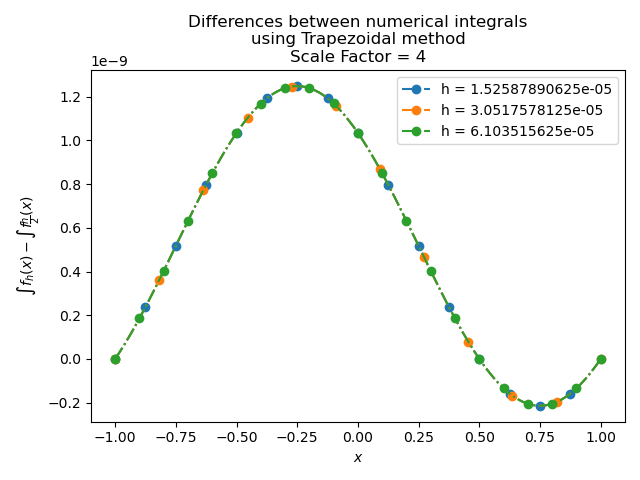
\includegraphics[width=0.7\linewidth]{figures/14-4-0.png}}
\caption{Effect of Step Size on Error Rate for Trapezoidal Rule}
\label{fig:14-4-0}
\end{figure}

\begin{figure}[H]
\centerline{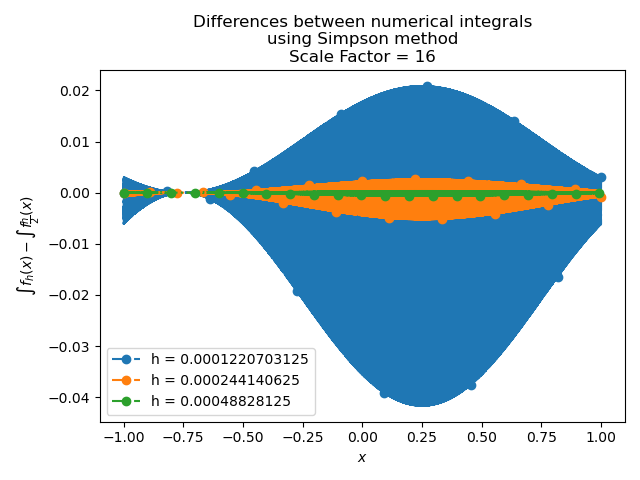
\includegraphics[width=0.7\linewidth]{figures/14-4-1.png}}
\caption{Effect of Step Size on Error Rate for Simpson's Method}
\label{fig:14-4-1}
\end{figure}

\section{Problem XV}

\subsection{Second Derivative Calculation}

\paragraph{} In the second derivative approximation, again, the centered difference with 3 point stencil is used. As can be seen from Figure \ref{fig:15-1}, this difference scheme is able to yield very accurate results. Also, from Figure \ref{fig:15-2}, the effect of step size on the error between succesive second derivative approximations can be seen. The discussion made about error types is also applicable for this case. The blue curve, which can be observed in Figure \ref{fig:15-2}, shows the instant when the round-off error starts to dominate.
\begin{figure}[H]
\centerline{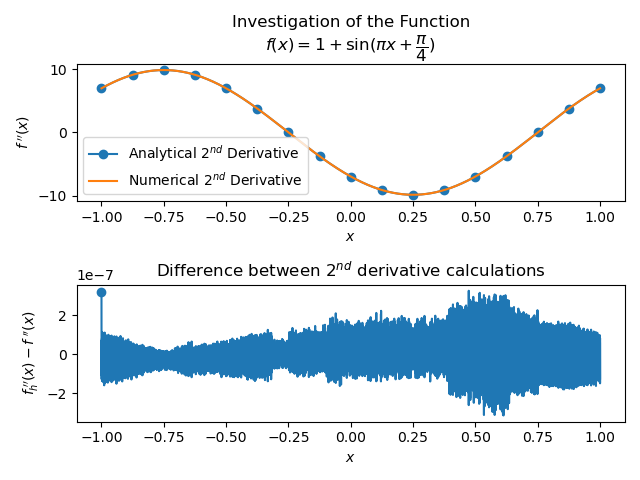
\includegraphics[width=0.8\linewidth]{figures/15-1.png}}
\caption{Analytical and Numerical Second Derivative of the Function}
\label{fig:15-1}
\end{figure}

\begin{figure}[H]
\centerline{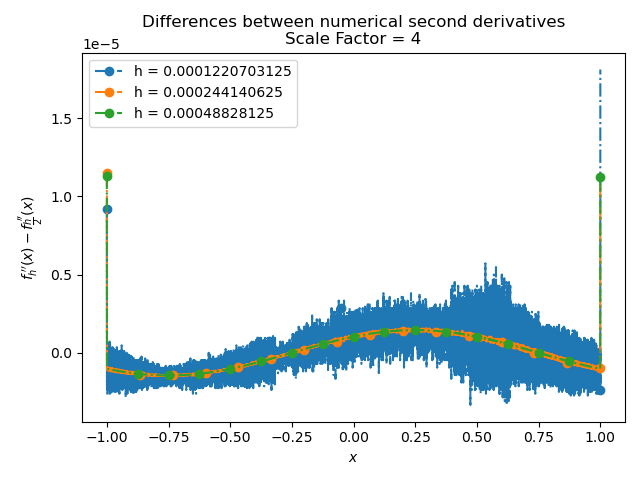
\includegraphics[width=0.7\linewidth]{figures/15-2.png}}
\caption{Effect of Step Size on Error Rate}
\label{fig:15-2}
\end{figure}

\subsection{Second Derivative as Two Successive First Derivative}
\paragraph{} Figure \ref{fig:15-3} shows the accomplishment of the second derivative approximation as two first derivative. Most of the time, it shows very small error rate for the approximation.
\paragraph{} As can be seen from Figure \ref{fig:15-3}, there are sharp fluctuations at the end. It is, doublessly, becuase of the fact when the first derivative is taken, the smooth transformations can be obtained, except the tip of functions. However, when another differentiation is executed, the smoothness at the tips is thoroughly spoiled. Therefore, the quite large differences at the tips are obtained. To be able to observe more accurate result, in Figure \ref{fig:15-3}, clipped version of the graph is provided.  
\begin{figure}[H]
\centerline{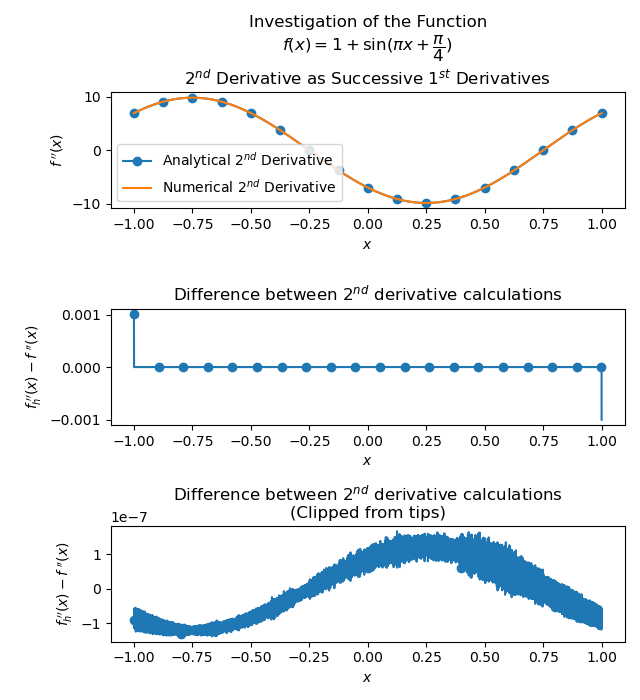
\includegraphics[width=\linewidth]{figures/15-3.png}}
\caption{Analytical and Numerical Second Derivative of the Function (Two First Derivatives)}
\label{fig:15-3}
\end{figure}


\label{sec:twofirstderiv}
\subsection{Integration Differentiation Inversion}
\paragraph{} Since the integration and differentiation is the inverse operator of each other's, we should be able to obtain the function itself after applying an integration and differentiation.  In Figure \ref{fig:15-4}, the result of the succesive application of numerical integration and differentiation can be observed. It, again, most of the time, yields very small error rate characteristics.
\paragraph{} The same discussion had in the Section \eqref{sec:twofirstderiv} can be applicable here. When there are more than one discretization operation, the readily discretized truncation error term starts to show its effect at the tips of the function. Therefore, again, in Figure \ref{fig:15-4}, the clipped version of the graph is provided.
\paragraph{} When the Figure \ref{fig:15-5-0} and Figure \ref{fig:15-5-1} are observed, the effect of the step-size and the integration rule can be investigated. As in all cases, the trapezoidal rule yields more smooth error characteristics compared to Simpson's rule. However, it is fact that the Simpson's rule is more inclined to yield less error compared to the Trapezoidal rule. 

\begin{figure}[H]
\centerline{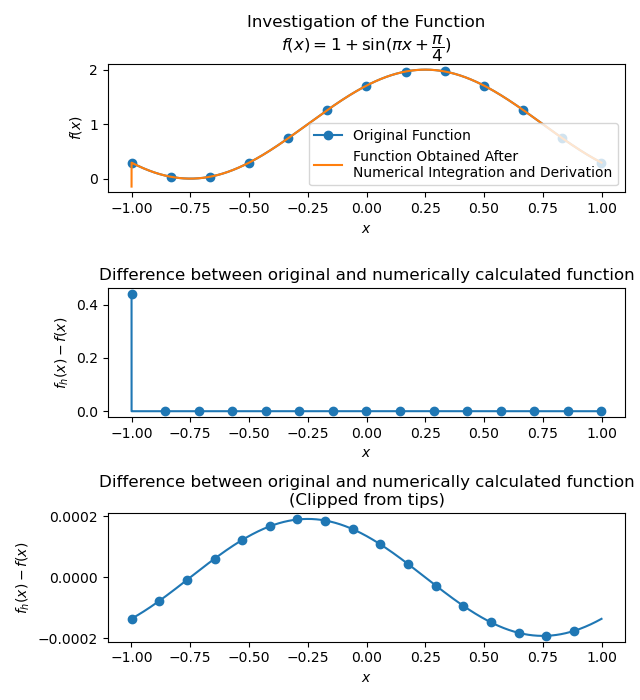
\includegraphics[width=0.8\linewidth]{figures/15-4.png}}
\caption{Integration Differentiation Inversion}
\label{fig:15-4}
\end{figure}


\begin{figure}[H]
\centerline{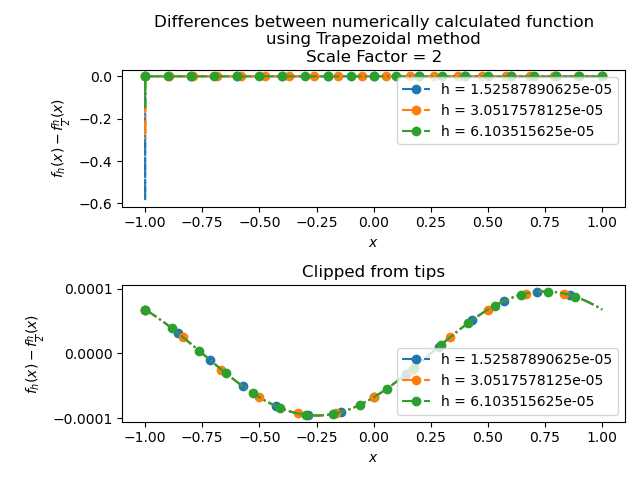
\includegraphics[width=0.7\linewidth]{figures/15-5-0.png}}
\caption{Effect of Step Size on Error Rate for Trapezoidal rule}
\label{fig:15-5-0}
\end{figure}

\begin{figure}[H]
\centerline{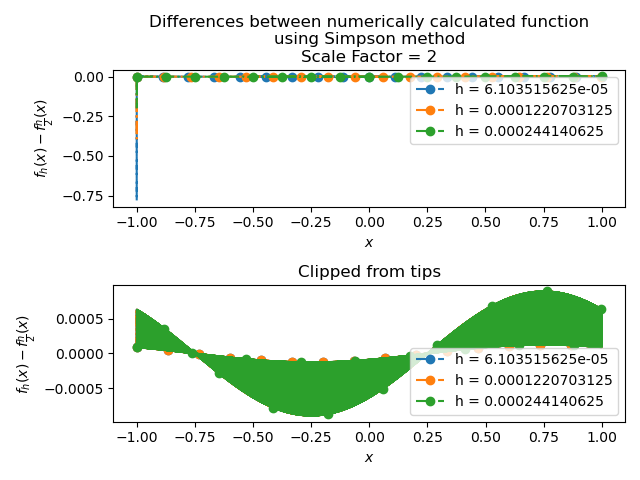
\includegraphics[width=0.7\linewidth]{figures/15-5-1.png}}
\caption{Effect of Step Size on Error Rate for Simpson's rule}
\label{fig:15-5-1}
\end{figure}

\pagebreak

\section{Problem XVI}
\subsection{Differentiation via using Arbitrary Data Points}
\paragraph{}As was discussed in Section \ref{sec:arbitstencil}, the stencils for an arbitrarily given data points can be found using \eqref{eq:stencileqnarb}.
\paragraph{} In this problem, previously used \textit{Hubble} data is analyzed. In Figure \ref{fig:16-1}, the derivative of the $d_L$ with respect to $z$ can be investigated. In Figure \ref{fig:16-1}, it can be also observed that the cubic spline derivative is intented to have a more exquisite behavior while the numerical derivative follows up more unruffled attitude.
\begin{figure}[H]
\centerline{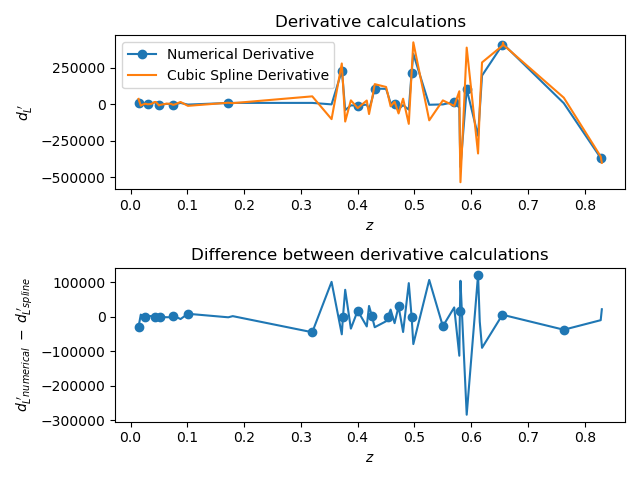
\includegraphics[width=\linewidth]{figures/16-1.png}}
\caption{Derivative of the Hubble Data }
\label{fig:16-1}
\end{figure}
\subsection{Integration via using Arbitrary Data Points}

\paragraph{} On the other hand, as can be observed in Figure \ref{fig:16-2}, the integration scheme displays a more consistent behavior. Overall, both the numerical integral and cubic spline integral intented to align with themselves. Therefore, in Figure \ref{fig:16-2}, the tightness between them can be asily observed.


\begin{figure}[H]
\centerline{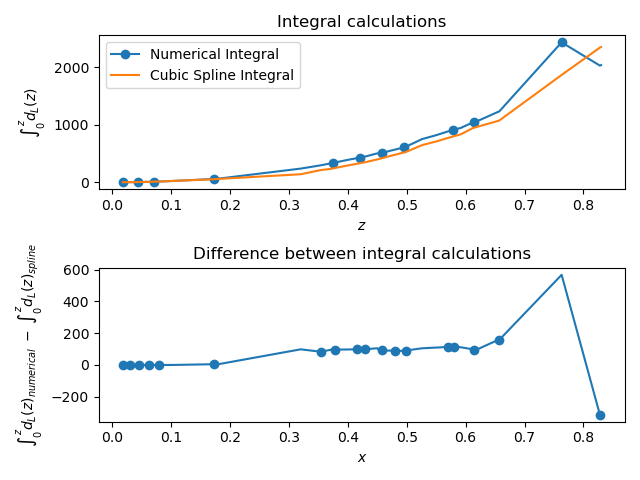
\includegraphics[width=1.0\linewidth]{figures/16-2.png}}
\caption{Integral of the Hubble Data}
\label{fig:16-2}
\end{figure}
\pagebreak
\subsection{Comparison of Implementation of Simpson's Methods}

\paragraph{} In the integration of \textit{Hubble} data, the composite Simpson's $1/3$ rule for an arbitrarily given data points is used. In Figure \ref{fig:16-3}, the time comparison between custom implementation and SciPy implementation can be observed. Figure \ref{fig:16-3} shows that the superiority of the readily implemented SciPy Simpson's function over the custom implementation. It, again, is again a neat indicator of the fact that \textit{we should always rely on the readily implemented packages when we are able to access it.}



\begin{figure}[H]
\centerline{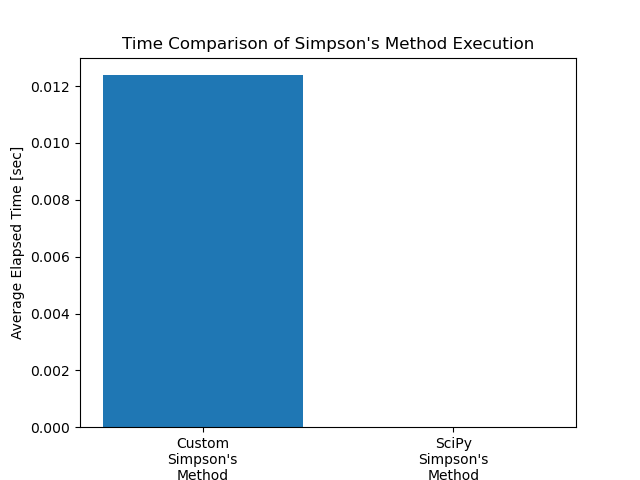
\includegraphics[width=1.0\linewidth]{figures/16-3.png}}
\caption{}
\label{fig:16-3}
\end{figure}

\paragraph{} Finally, in Figure \ref{fig:16-4}, the comparison between custom Simpson's method implementation and SciPy implementation can be observed. It can be concluded that the custom implementation and SciPy implementation well align until a certan point, therefore, the overall difference between them is low.
\begin{figure}[H]
\centerline{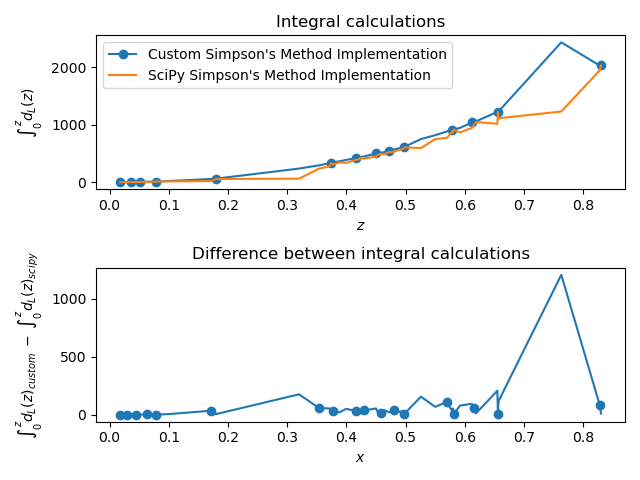
\includegraphics[width=\linewidth]{figures/16-4.png}}
\caption{Integral calculation using Simpson's method}
\label{fig:16-4}
\end{figure}


\section{Problem XVII}
\subsection{Gaussian Quadrature Implementation}
\paragraph{} In this problem, the integration calculation is made via using \textit{Gaussian quadrature}. In Figure \ref{fig:17-1}, the result of the integration can be observed for different degrees of quadrature.
\begin{figure}[H]
\centerline{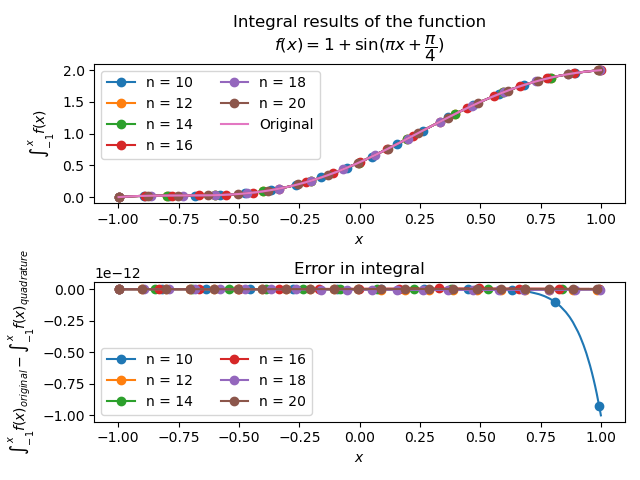
\includegraphics[width=\linewidth]{figures/17-1.png}}
\caption{Integral calculation using Gaussian Quadrature}
\label{fig:17-1}
\end{figure}

\end{document}

              


